% SW design
\clearpage

\section{Software design}

Design fasen var mere eller mindre lige til efter alt den foreliggende dokumentation var på plads. Opgaverne blev delt ud således at Jesper lavede PC delen, Bjørn lavede software til senderen og Jeppe til modtageren og ClickATell klassen. Vi har løbende haft møder og forsøgt at hjælpe hinanden når der var nogle spørgsmål.

\subsection{PC delen (JC)}

Softwaren til PC'en, er brugeren grænseflade til at kontrollere systemet. Her kan han manurære rundt i de forskellige menuer og udføre de forskellige ting som er beskrevet i use casene.

Nedenfor er der illustreret hvordan man kommer frem og tilbage i brugerinterfacet. Udover bruger input så kan CSS hovedenheden give PC'en besked om at der ikke længere er logget ind hvilket vil sende brugeren fra main menu og tilbage til pre-login menuen.

\begin{figure}[htbp] \centering
{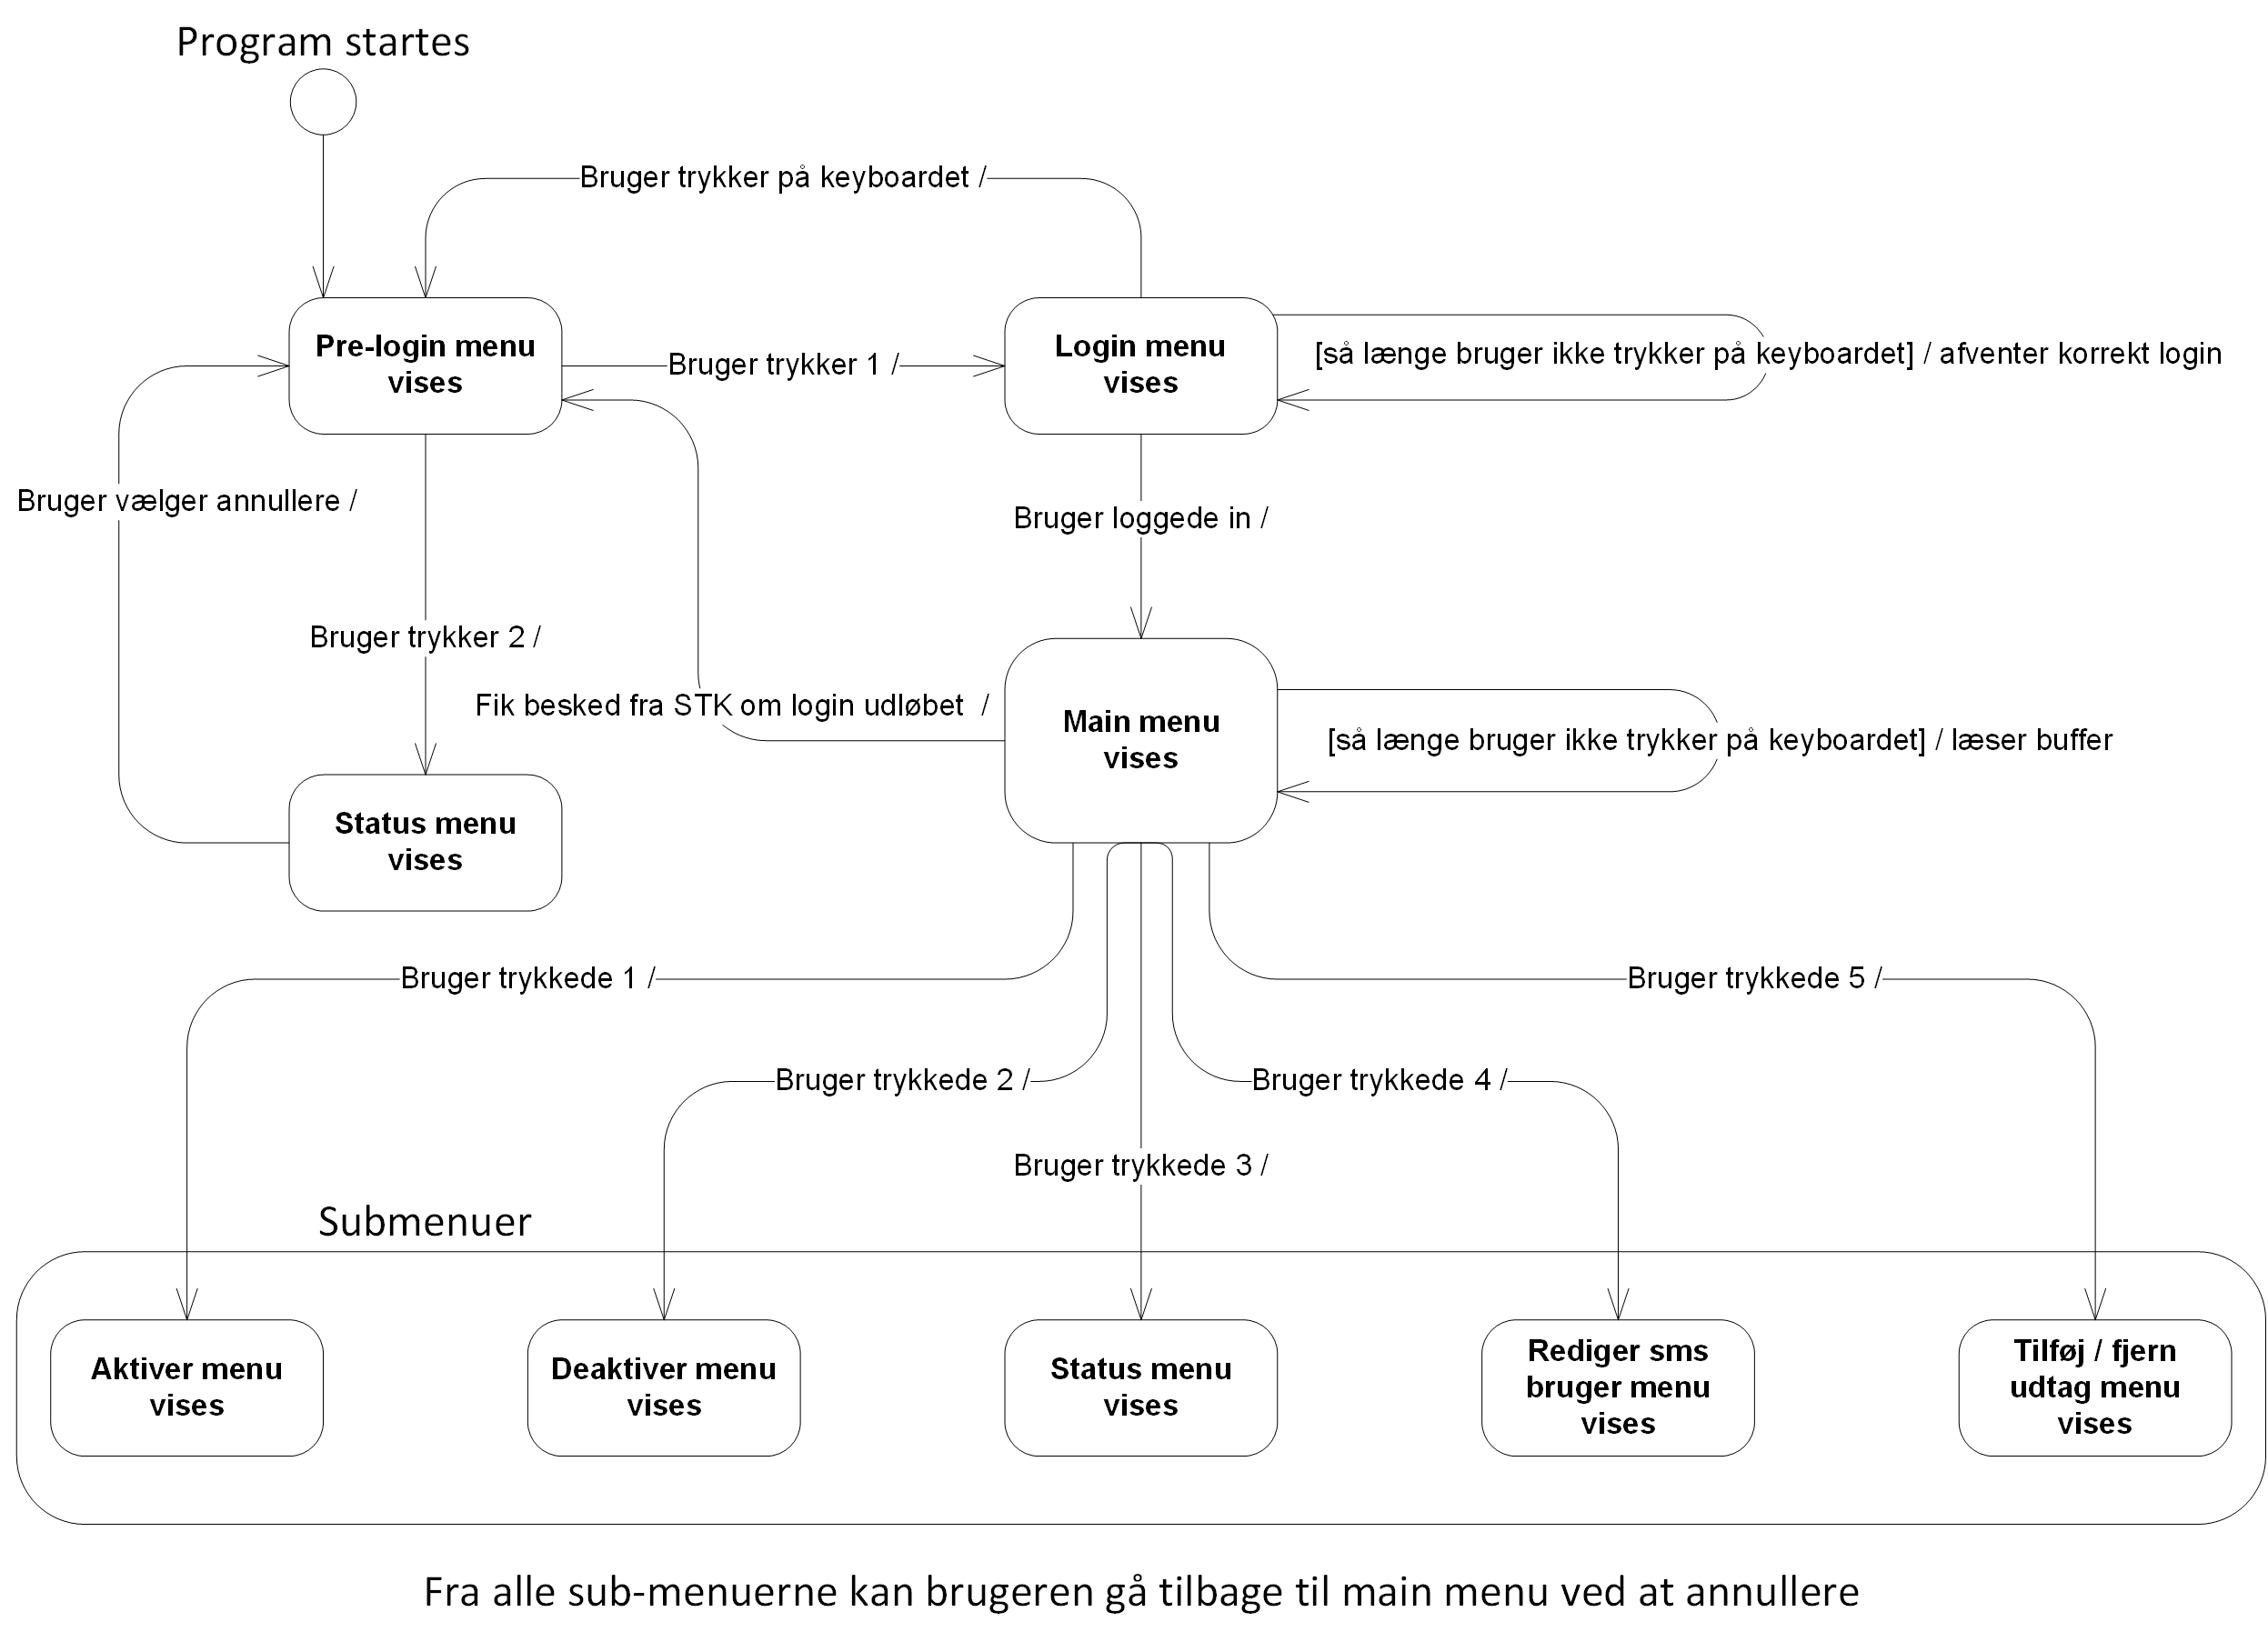
\includegraphics[width=\textwidth]{billeder/uml/state_machine_main}}
\caption{State machine diagram over brugerflade}
\label{lab:State machine diagram over brugerflade}
\end{figure}